\section{Software - \AndreasGrain}
Im Zuge dieser Diplomarbeit wurden folgende Software-Teile programmiert:
\begin{itemize}
    \item Oberfläche der Applikation (PiBell/MainPage.xaml)
    \item Klassen zur Verwaltung der Dienste (PiBell/Classes/MediaClasses.cs)
    \item Berechtigungsmanagement (PiBell.Android/MainActivity.cs)
    \item Audio-Aufnahme-Service in Android (PiBell.Android/AudioRecordingService.cs)
    \item Audio-Aufnahme-Service in iOS (PiBell.iOS/AudioRecordingService.cs)
\end{itemize}

\begin{figure}[htbp!]
    \centering
    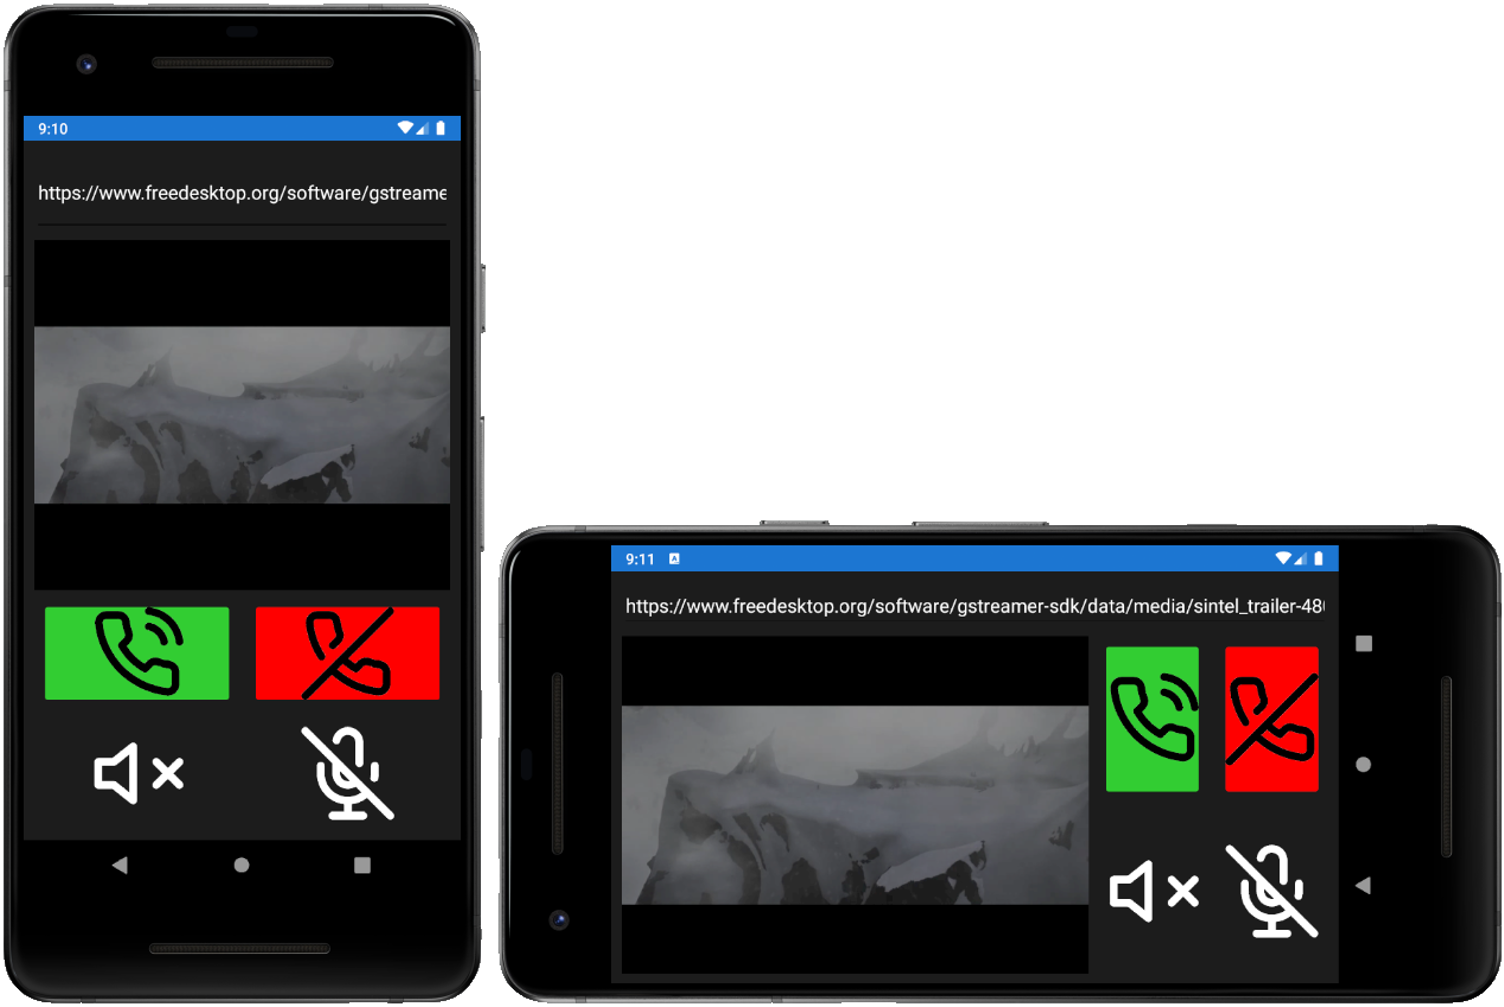
\includegraphics[width=.9\linewidth]{images/projektergebnis/ansichtenFinaleApp.png}
    \caption{App-Ansichten}
\end{figure}

Aus diesen Software-Teilen wurde eine fertige Android-Applikation erstellt, mit der der Fernzugriff auf die fest installierte Videosprechanlage jederzeit möglich ist.
Die Kommunikation wurde bidirektional für die Ton- und unidirektional für die Video-Übertragung realisiert.
Die Applikation wurde auf verschiedenen Systemen simuliert und in geringem Ausmaß getestet.
Eine iOS-Version wurde aufgrund fehlender Endgeräte nicht fertiggestellt bzw. getestet.\par

Die programmierte Applikation ist in diesem Dokument ausführlich beschrieben und wesentliche Funktionen im Detail erklärt.
Die Erläuterung des Programm-Codes ist kein Ersatz für das Sprach-Regelwerk des Herstellers, sondern ein Kommentar wie der Autor \AndreasGrain\ dieses versteht!
Im Zweifelsfall wird darauf hingewiesen, dass die offiziellen Angaben der Hersteller zu verwenden sind.
Auf diese wird an relevanten Stellen verwiesen.

Verwendete Technologien und Software:
\begin{itemize}
    \item \ac{rtsp} zur Übertragung der Mediendaten über das Netzwerk
    \item LibVLC Sharp zum Abrufen und Darstellen des Video-Streams
    \item GStreamer zur Weiterverarbeitung der Mediendaten am Server
    \item Live555 Proxy zum Verteilen des \ac{rtsp}-Streams
    \item Push Benachrichtigung zur Kontaktaufnahme mit dem Benutzer der App
    \item Visual Studio 2019 als Entwicklungsumgebung
    \item Xamarin-Rahmenwerk für die Entwicklung der Multiplattform-App
    \item \hologo{XeLaTeX} zur Erstellung der Dokumentation
\end{itemize}

\section{Hardware - \MatthiasMair}
Im Zuge der Diplomarbeit wurde eine Einzel-\ac{smd}-Platine entwickelt, welche den internen Aufbau der Sprechanlage-Stationen vereinfacht.
Die neu entwickelte Platine ersetzt folgende Bausteine der bisherigen Stations-Hardware:
\begin{itemize}
    \item Spannungsregler zur Versorgung der Komponenten
    \item Lautsprecherverstärker zur Verstärkung des Lautsprechersignals
    \item Mikrofonverstärker zur Vorverstärkung des Mikrofon-Tons
\end{itemize}
Zusätzlich zu den alten Funktionen beinhaltet die neue Platine einen Watchdog-Timer, welcher die Betriebsstabilität der Station überwacht.

\begin{center}
	\begin{minipage}[t]{0.475\linewidth}
		\begin{figure}[H]
			\centering
			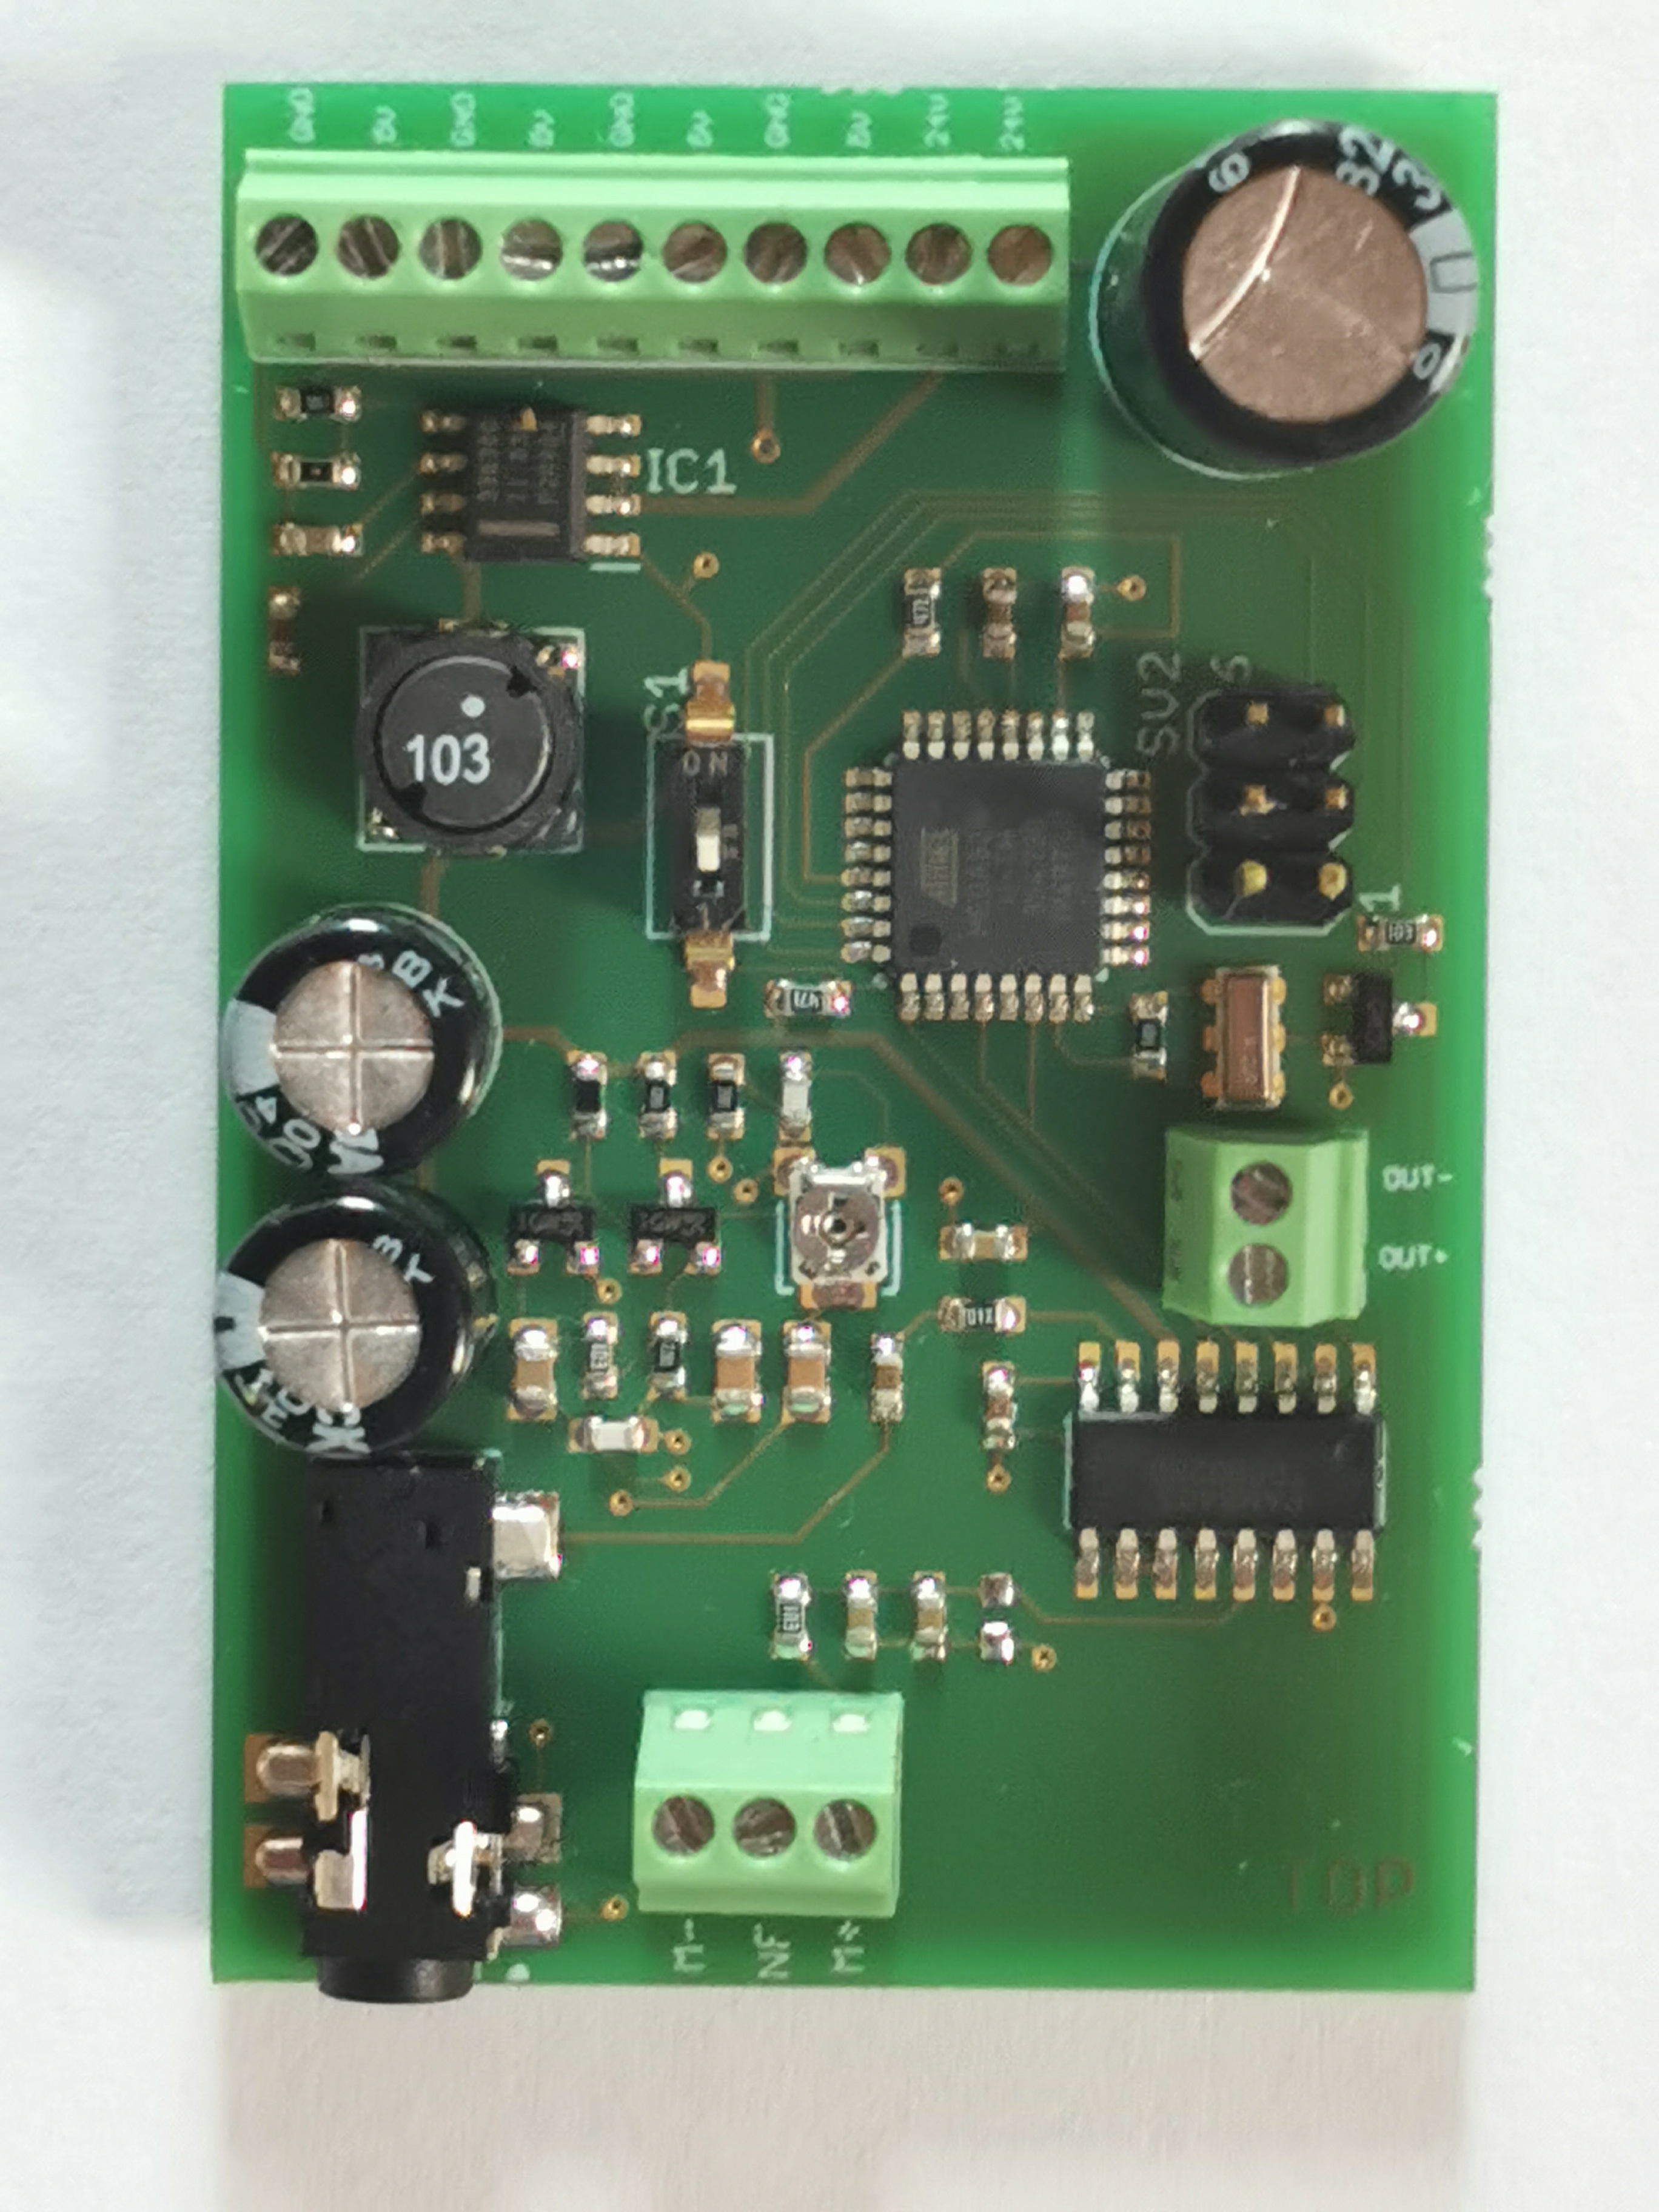
\includegraphics[width=\textwidth]{images/projektergebnis/platineV1top.jpg}
			\caption{Bestückte Platine Top}
		\end{figure}
	\end{minipage}
	\begin{minipage}[t]{0.475\linewidth}
		\begin{figure}[H]
			\centering
			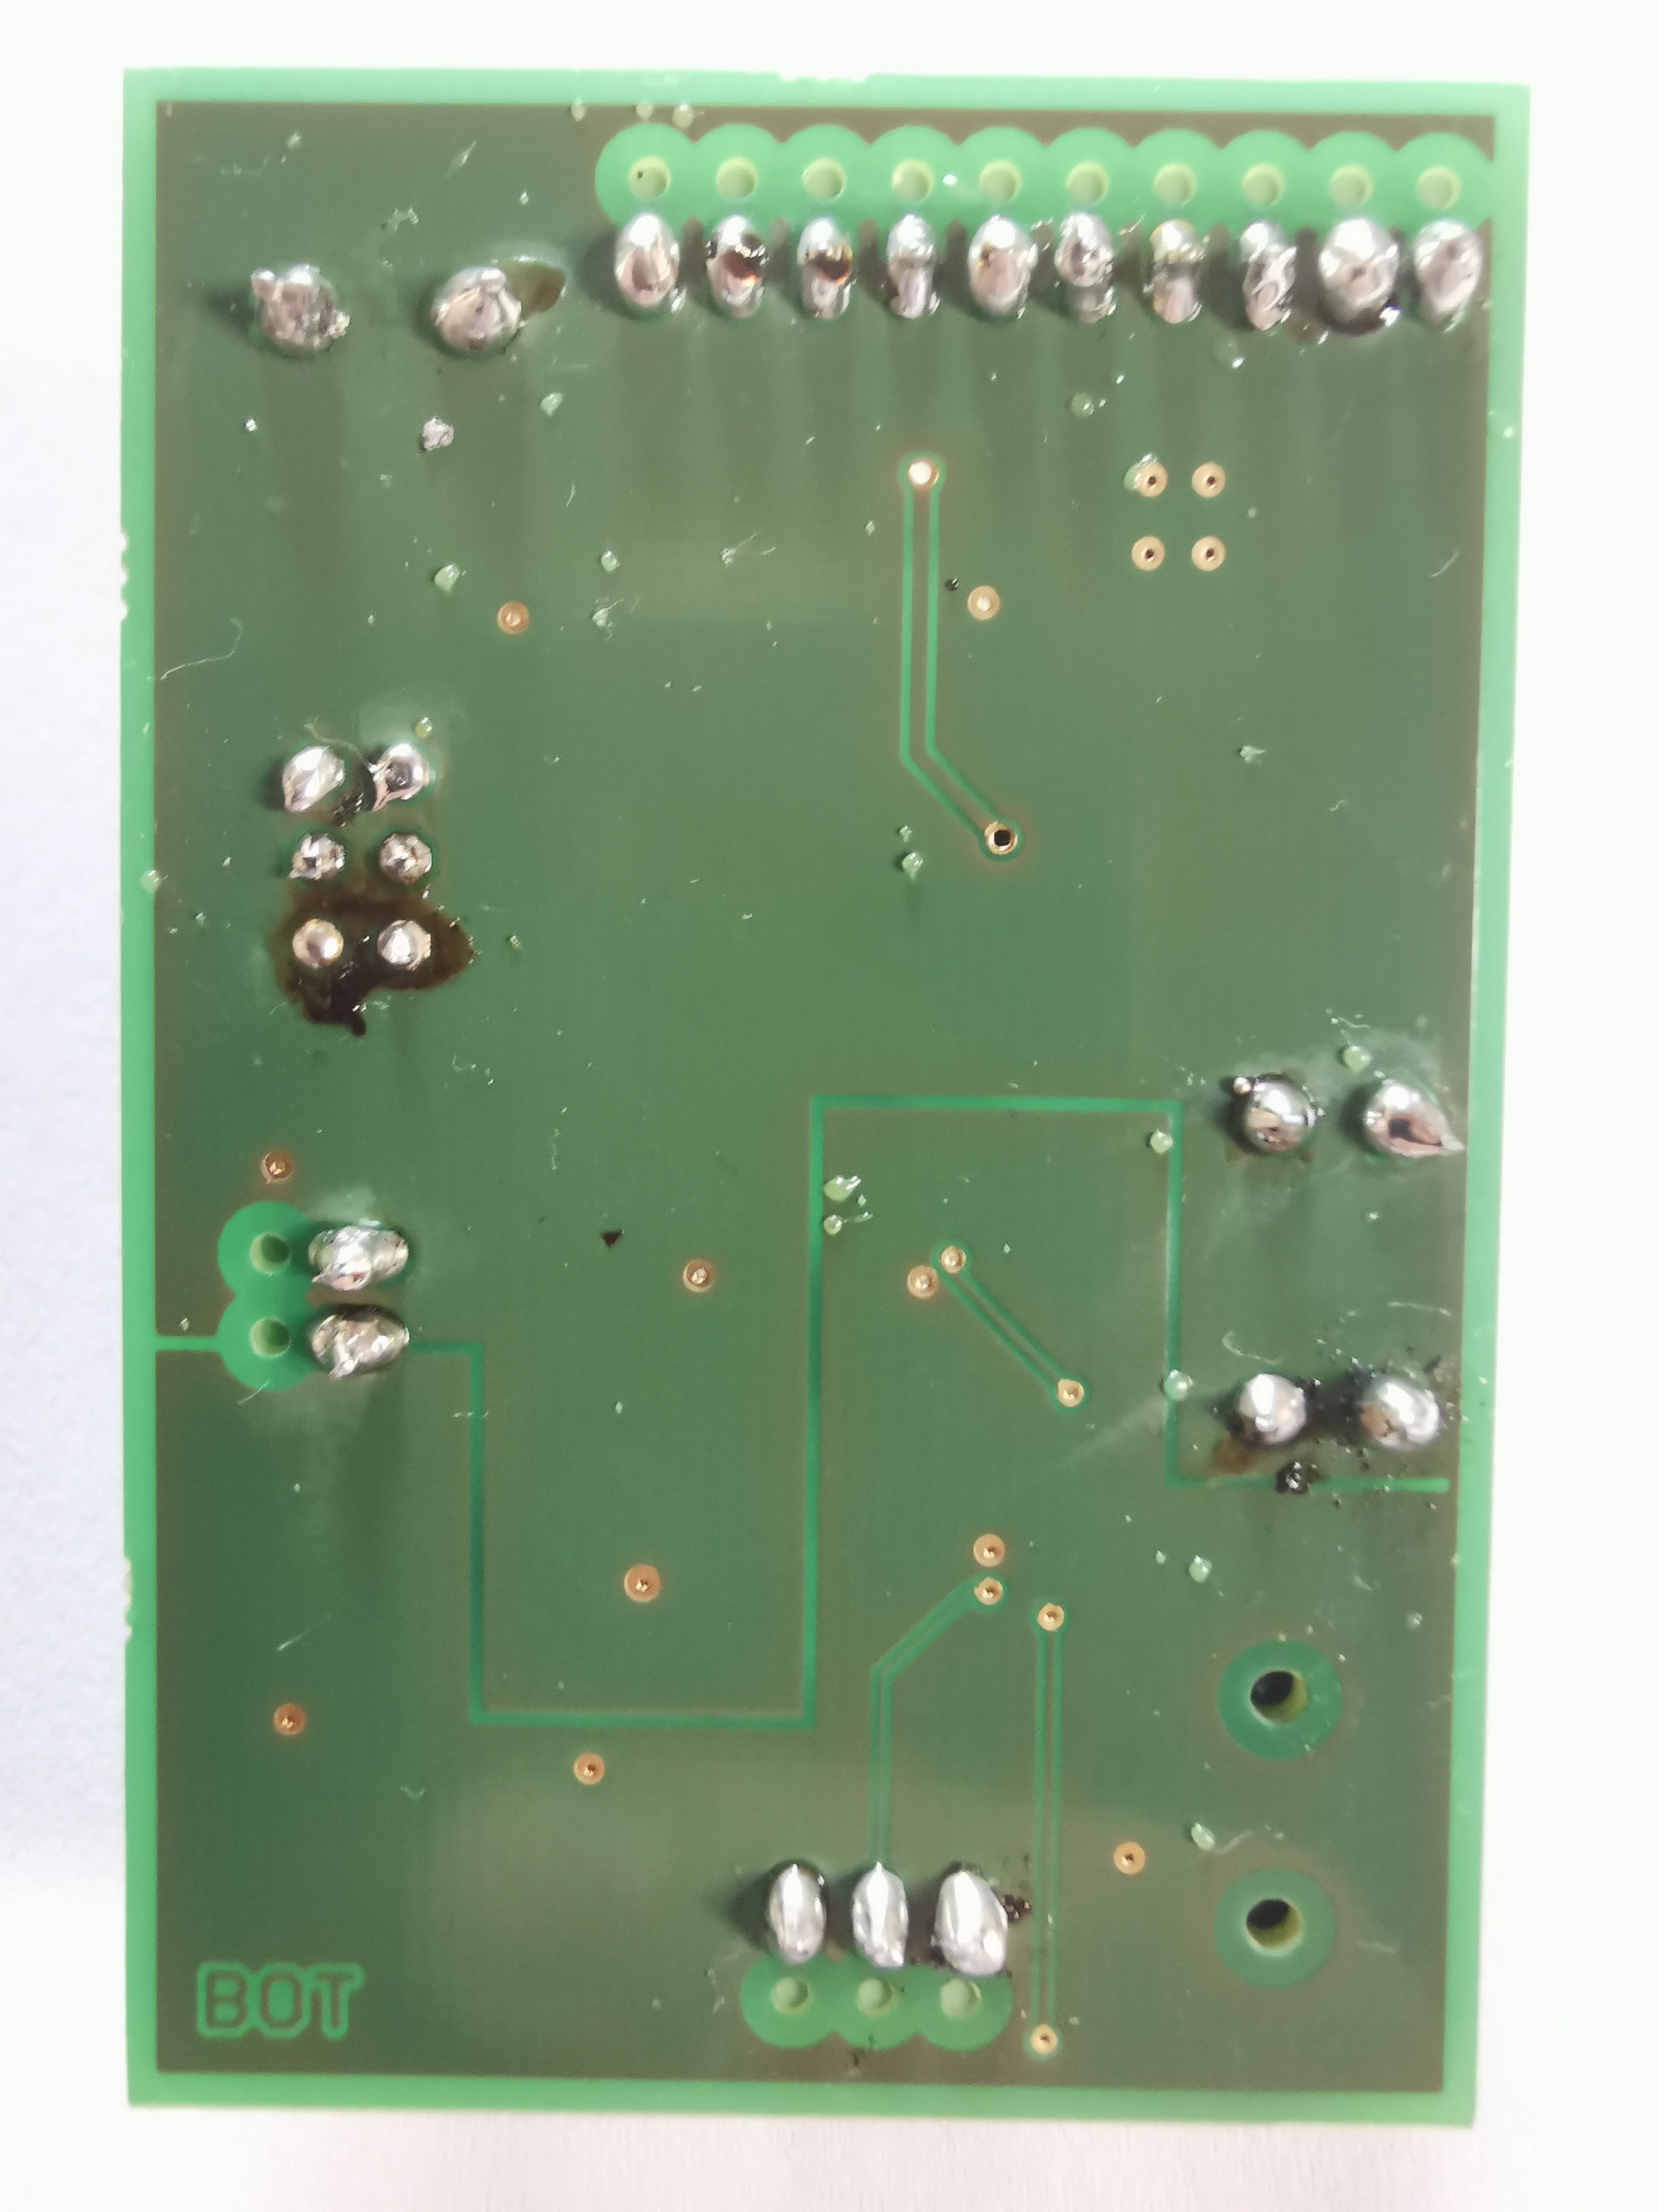
\includegraphics[width=\textwidth]{images/projektergebnis/platineV1bot.jpg}
			\caption{Bestückte Platine Bottom}
		\end{figure}
	\end{minipage}
\end{center}

Die Bestellung der Platine und der Großteil der Bestückung dieser erfolgte über \MarioPrantl s Firma Mario Prantl Solutions.
Die Vervollständigung der Platine durch Einlöten der \ac{tht}-Komponenten erfolgte per Hand durch \MatthiasMair.

Verwendete Technologien und Software:
\begin{itemize}
    \item \ac{eagle} zur Erstellung des Schaltplans und Planung des Platinen-Layouts
    \item Arduino \ac{ide-dev} zur Programmierung des Mikrocontrollers
\end{itemize}

Im Zuge der Diplomarbeit wurde eine zweite Version der Platine entwickelt.
Diese verfügt über zusätzliche Anschlusspunkte, welche mit digitalen \acp{io} des Mikrocontrollers verbunden sind.
Die Platine ist vollständig geplant, konnte allerdings aufgrund der COVID-19-Krise in Tirol nicht im festgelegten Zeitrahmen gefertigt werden.